En esta sección se detallan las páginas web asociadas a \textif{Feed the Realm} desarrolladas, el objetivo de su creación y qué características principales
tienen las mismas, entre otros detalles de implementación.

\subsubsection{Backoffice}

Se implementó una página web utilizando \textit{React} y \textit{Typescript} para uso administrativo por parte del equipo de desarrollo,
con el objetivo de reducir tiempos de operaciones manuales como lo pueden ser lanzar o apagar un 'zoning server' manualmente,
cambiar el balance de gemas de un usuario en específico o incluso llevar a cabo el \textit{Release} de una nueva versión de alguna de las aplicaciones.

Esta página hace uso de varios \textit{endpoints} protegidos del \textit{Core-service} y de exclusivo acceso para administradores, 
como también tiene acceso al CDN para poder obtener y visualizar cosméticos ligados a un mundo o a un usuario.

\paragraph{Dashboard}

Luego de pasar por el proceso de login como administrador, se entra a la vista general del estado del juego. Esta cuenta con métricas generales y estados de los servicios como:

\begin{itemize}
    \item Cantidad total de usuarios registrados en el sistema.
    \item Cantidad de usuarios activamente jugando (conectados a algún mundo) y duración promedio de una sesión de juego.
    \item Ratio de mundos y zonas \textit{online} versus \textit{offline}.
    \item Flujo de gemas y métricas de la economía de los cosméticos.
    \item Balance total de todos los creadores de mundos.
\end{itemize}

\begin{figure}[H]
    \centering
    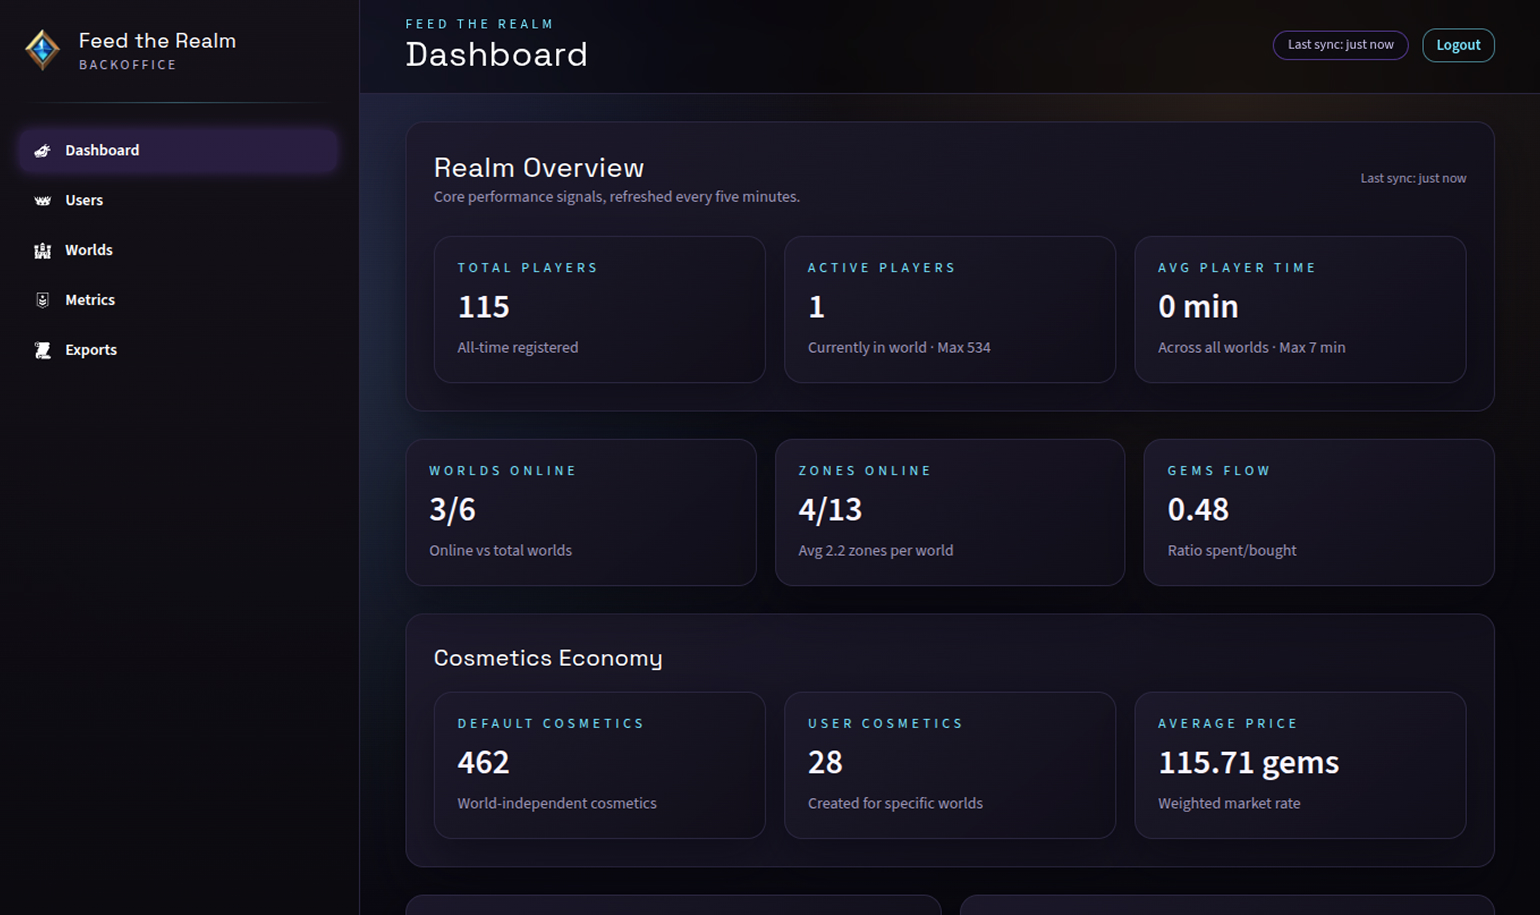
\includegraphics[width=1\textwidth]{img/08-implemented-solution/websites/bo-dashboard.jpg}
    \caption{Captura del Dashboard del Backoffice.}
\end{figure}

\paragraph{Usuarios}

En esta vista se pueden observar todos los usuarios existentes de forma paginada, ver sus detalles, actualizar su cantidad de gemas,
otorgar privilegios de administrador o realizar búsquedas por email o estados (verificado/sin verificar/todos).

Dentro de los detalles de usuario se encuentran, su balance de gemas como jugador y \textit{USD} como creador (basado en las ventas de cosméticos ocurridas en un mundo creado por el mismo),
sus cosméticos comprados y también sus cosméticos equipados o en uso.

\begin{figure}[H]
    \centering
    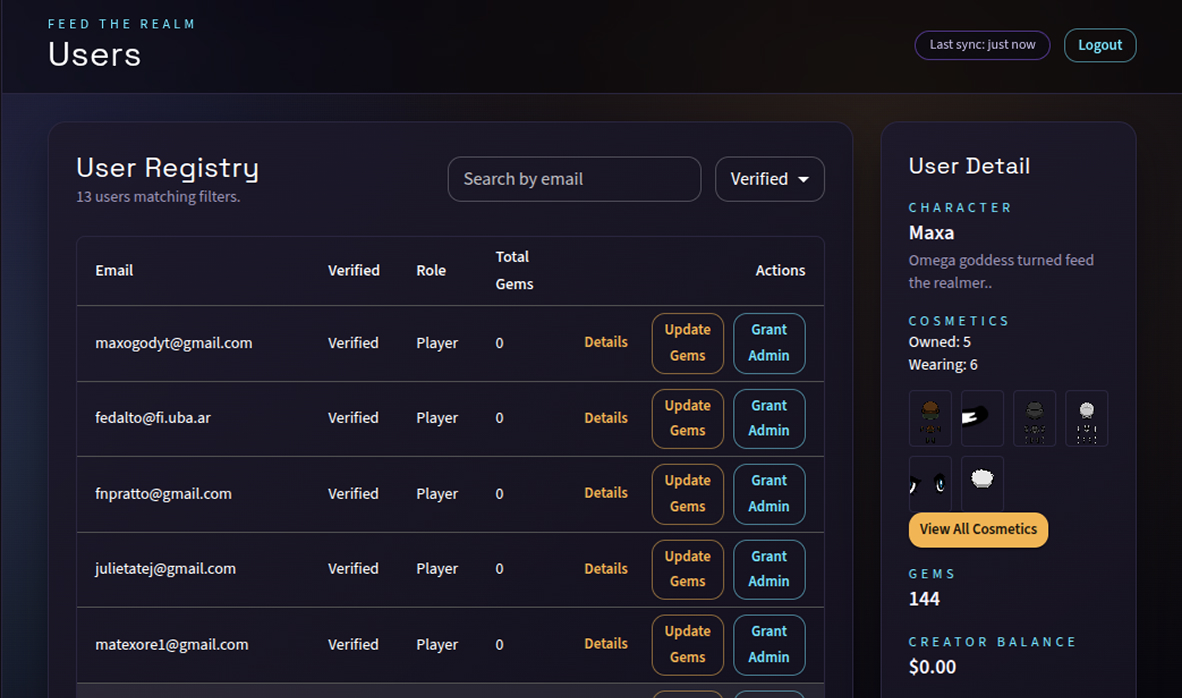
\includegraphics[width=0.85\textwidth]{img/08-implemented-solution/websites/bo-users.jpg}
    \caption{Captura de la sección de usuarios del Backoffice.}
\end{figure}

\paragraph{Mundos}

En la vista de los mundos se tiene la lista paginada de todos los mundos creados, que al igual que con los usuarios se pueden buscar por nombre
o filtrar por estados, en este caso \textit{online}, \textit{offline} o \textit{degraded} (tiene al menos una zona activa, pero fuera de servicio).

Adicionalmente, cada entrada de la lista cuenta con los detalles de dicho mundo, donde se pueden ver métricas generales como cantidad de jugadores
activos actualmente y tiempo promedio de juego, la lista de cosméticos creados y la lista de zonas existentes con sus direcciones en caso de estar \textit{online} y
con la posibilidad de lanzar o parar los \textit{Nomad jobs} correspondientes a las mismas.

\begin{figure}[H]
    \centering
    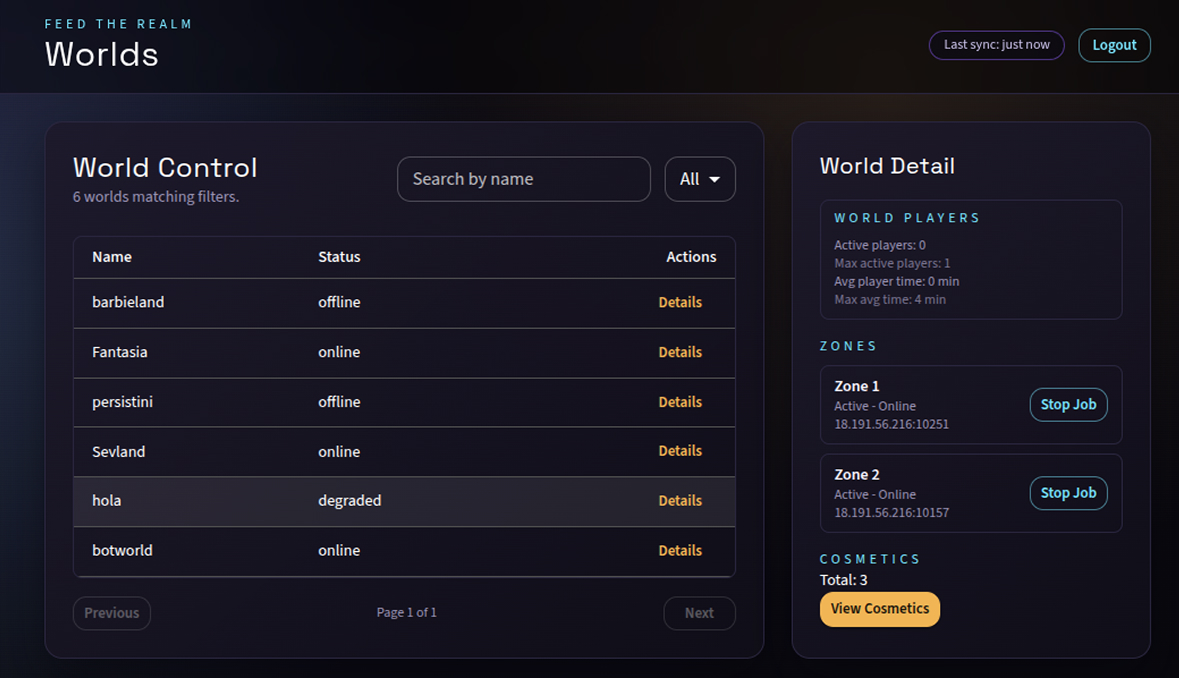
\includegraphics[width=0.85\textwidth]{img/08-implemented-solution/websites/bo-worlds.jpg}
    \caption{Captura de la sección de mundos del Backoffice.}
\end{figure}

\paragraph{Métricas}

Luego se tiene la vista asociada a métricas de negocio más detalladas, varias las cuales se muestran también en la sección del \textit{Dashboard}.

Dentro de las mismas se encuentran otras adicionales, como lo puede ser el promedio de zonas por mundo, la ganancia total de \textit{Feed the Realm}
obtenida por la venta de gemas y el precio promedio en gemas de los cosméticos.

\begin{figure}[H]
    \centering
    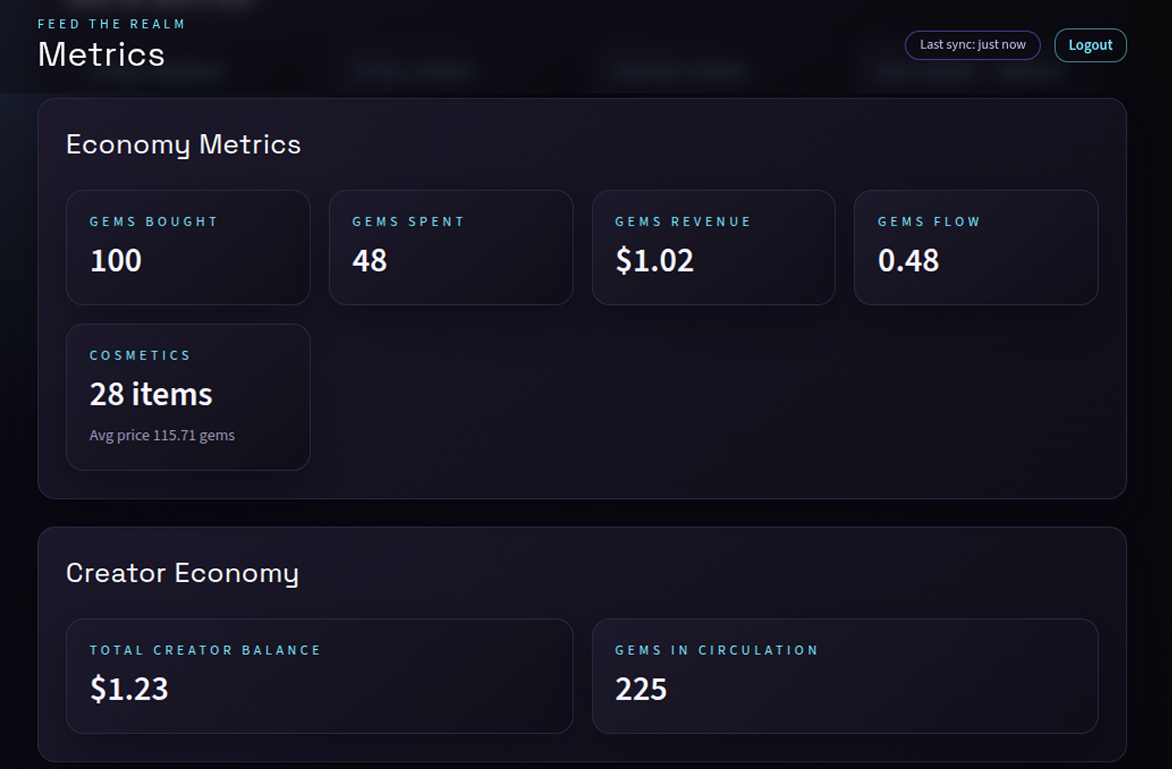
\includegraphics[width=0.7\textwidth]{img/08-implemented-solution/websites/bo-metrics.jpg}
    \caption{Captura de la sección de métricas del Backoffice.}
\end{figure}

\paragraph{Publicación de \textit{Releases}}

Finalmente, la vista de \textit{Exports} es la utilizada por los administradores para publicar nuevas versiones de las aplicaciones 'Cliente' para
los diferentes sistemas operativos soportados.

Para llevar a cabo una publicación una vez se tiene el archivo comprimido de la aplicación compilada, se selecciona el tipo de la misma, esto puede ser
\textbf{Feed the Realm - Game} o \textbf{Feed the Realm - World Editor}, y luego se le asigna un nombre de versión, un sistema operativo para el cual
se compiló y el archivo en cuestión.

Una vez hecha la publicación, se la puede marcar con la etiqueta \textit{latest}, y a partir de ese momento las próximas descargas del juego o editor de mundos
obtendrán la nueva versión.

\begin{figure}[H]
    \centering
    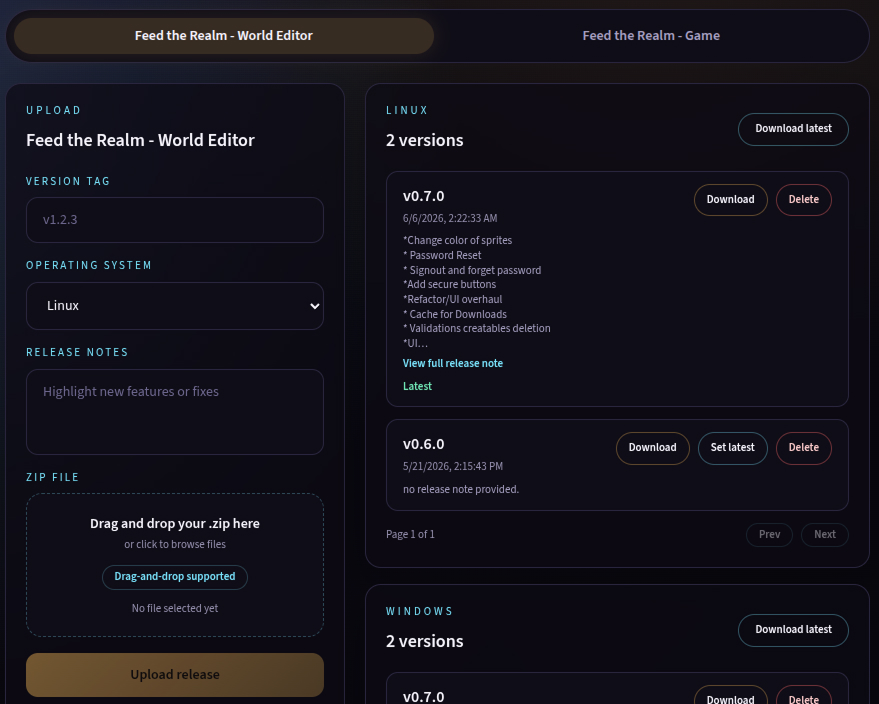
\includegraphics[width=0.7\textwidth]{img/08-implemented-solution/websites/bo-exports.jpg}
    \caption{Captura de la sección de \textit{exports} del Backoffice.}
\end{figure}

\subsubsection{Landing page}

Se implementó una segunda página web utilizando \textit{React} y \textit{Typescript} de libre acceso, con el objetivo de publicar
información sobre \textit{Feed the Realm}, detalles de su desarrollo, videoclips e imágenes y opciones de descarga de las aplicaciones a
modo de \textit{onboarding} para nuevos posibles usuarios.

Esta página es mayormente estática, pero hace uso de los \textit{endpoints} de lectura del \textit{Core-service} relacionados con los \textit{Releases} de cada aplicación, 
como también hace uso del CDN para poder descargar los archivos.

\begin{figure}[H]
    \centering
    
\includegraphics[width=0.85\textwidth]{img/08-implemented-solution/websites/landing-home.jpg}
    \caption{Captura del home de la landing page.}
\end{figure}

\vspace{0.25cm}

Las características principales de esta página son:

\begin{itemize}
    \item \textbf{Home}: Contiene una corta descripción del juego, un resumen del resto de secciones y enlaces de interés como lo son los de descarga de las aplicaciones para 
    el sistema operativo deseado, el del canal de \textit{youtube} y el del servidor de \textit{discord} de la comunidad, entre otros.
    \item \textbf{Media}: Contiene una galería de imágenes y videos del juego a modo de vista general con motivos de capturar el interés de posibles jugadores.
    \item \textbf{Blog}: Página de blogs para avisos de nuevas versiones, cambios o \textit{features} a lo largo del desarrollo y ciclo de vida del juego.
\end{itemize}

\begin{figure}[H]
    \centering
    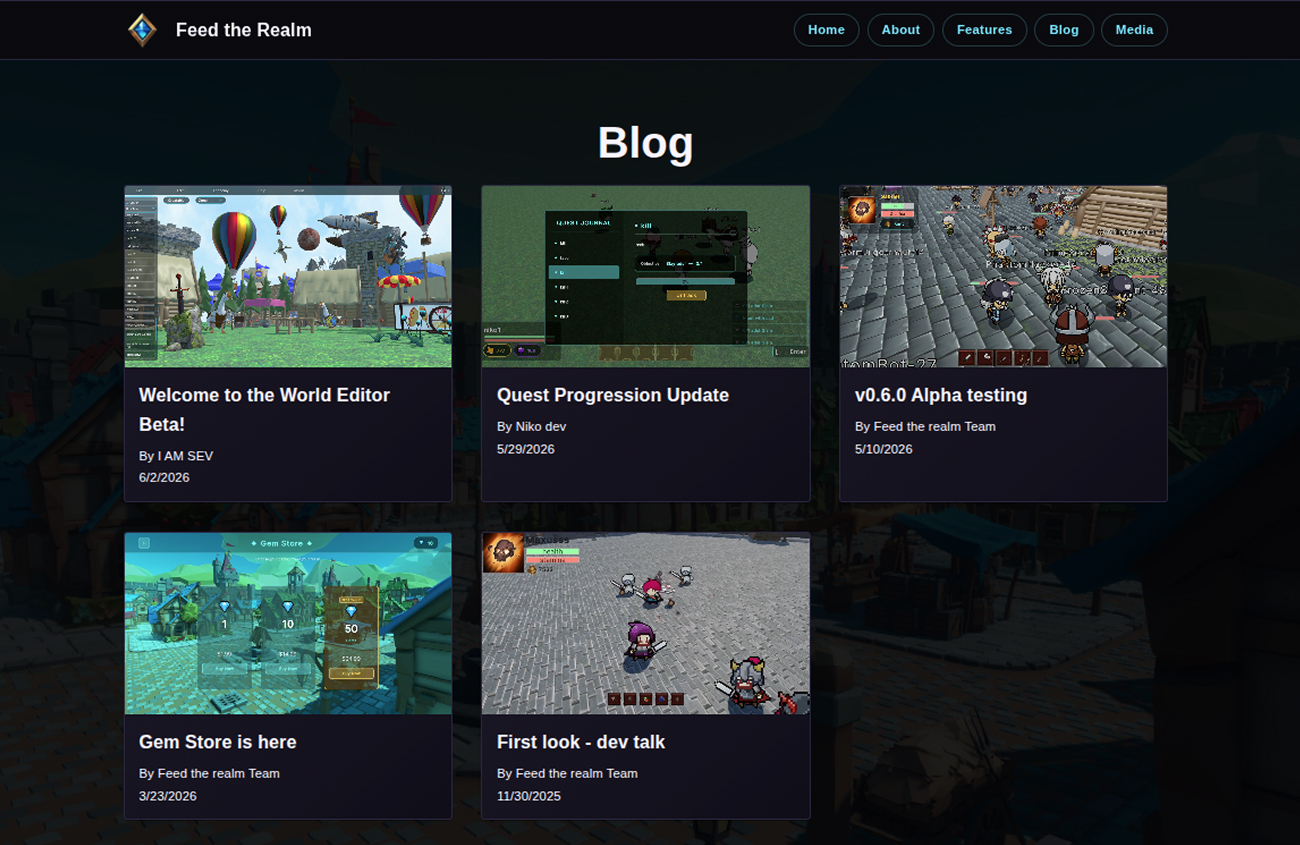
\includegraphics[width=0.85\textwidth]{img/08-implemented-solution/websites/landing-blog.jpg}
    \caption{Captura de la sección de blog de la landing page.}
\end{figure}
